% !TEX encoding = UTF-8 Unicode
% !TEX TS-program = xelatex

\documentclass{article}
	\usepackage[cm]{fullpage}
	\usepackage{fontspec}
	\setmainfont{SourceCodePro-Regular}
	\usepackage{tikz}
	\usepackage{listings}
\begin{document}

	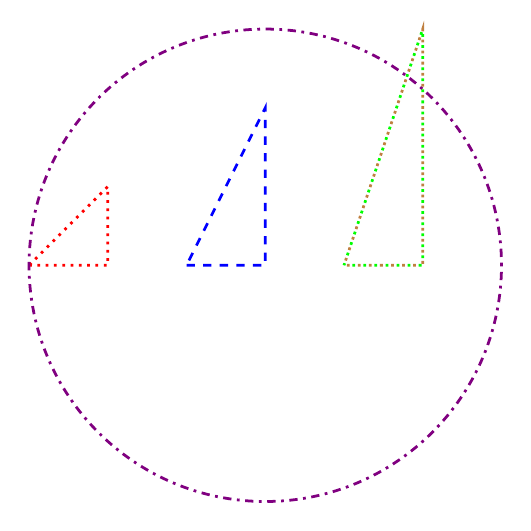
\begin{tikzpicture}[line width = 1pt]
		\draw [red, dotted] (0,0) -- (1,0) -- (1,1) -- (0,0);
		\draw [blue, dashed] (2,0) -- (3,0) -- (3,2) -- (2,0);
		\draw [violet, dash pattern = on 1pt off 2pt on 3pt off 2pt]
			(3,0) circle[radius = 3];
		\newcommand\thintriangle{(4,0) -- (5,0) -- (5,3) -- (4,0)}
		\draw [green, dash pattern = on 1pt off 3pt, dash phase = 1pt] \thintriangle;
		\draw [brown, dash pattern = on 1pt off 3pt, dash phase = 3pt] \thintriangle;
	\end{tikzpicture}

\lstset{language=[latex]tex,tabsize=4}
\lstset{moretexcs={draw}}
\begin{lstlisting}
% !TEX encoding = UTF-8 Unicode
% !TEX TS-program = pdflatex
\documentclass{article}
	\usepackage{tikz}
\begin{document}
	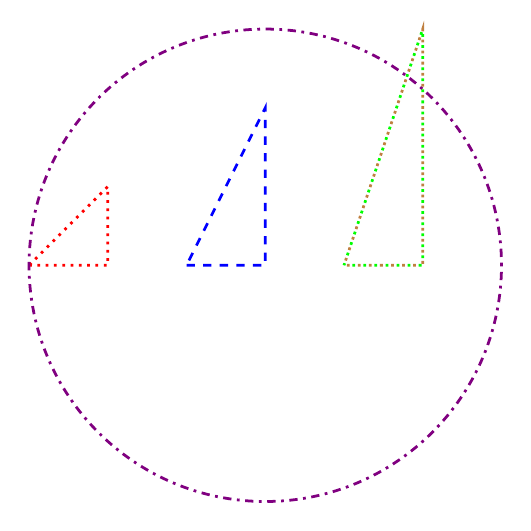
\begin{tikzpicture}[line width = 1pt]
		\draw [red, dotted] (0,0) -- (1,0) -- (1,1) -- (0,0);
		\draw [blue, dashed] (2,0) -- (3,0) -- (3,2) -- (2,0);
		\draw [violet, dash pattern = on 1pt off 2pt on 3pt off 2pt]
				(3,0) circle[radius = 3];
		\newcommand\thintriangle{(4,0) -- (5,0) -- (5,3) -- (4,0)}
		\draw [green, dash pattern = on 1pt off 3pt,
				dash phase = 1pt] \thintriangle;
		\draw [brown, dash pattern = on 1pt off 3pt,
				dash phase = 3pt] \thintriangle;
	\end{tikzpicture}
\end{document}
\end{lstlisting}

\end{document}